\section{Noise Generation}
\label{section:noise}
Nature's chaotic and fortuitous behavior creates a world full of diversity and unpredictability.
This can be observed in a surprisingly high amount of objects, structures and phenomenons.
\\
For example, the following images show photographs of patterns that seem almost completely random.

\begin{figure}[H]
    \includegraphics[width=\linewidth]{nature-random.png}
    \caption{Random pattern observed in Nature \protect\cite{bookofshaders:noise}.}
    \label{img:rnd:natural}
\end{figure}

\noindent
In computer science, the virtual recreation of such randomness has been studied continuously over the last decades.
The outcome of a randomness generator is called \emph{\gls{noise}}.
There are many established algorithms to create random patterns, one of which is the famous \emph{Voronoi} algorithm.

\subsection{Previous Work}
Many of the following subsections rely on concepts and algorithms that have been thorougly explained in the project's previous work \cite{project2:noise}.
This include sine-based deterministic number generation algorithms, also known as also \emph{\gls{pseudorandom}} number generation \cite{project2:noise:pseudo}.
It further includes different \gls{noisegeneration} algorithms like Perlin \gls{noise} \cite{project2:noise:perlin}.
\emptyline
Those algorithms will not be described again, as they have already been studied and documented before.

\pagebreak

\subsection{Voronoi's Algorithm}
\label{section:noise:voronoi}
One of the more commonly used procedural pattern generation algorithms is that of Steven Worley, developed in 1996 \cite{worley}.
The name derives from its similar structure to a Voronoi diagram, in which points, called \emph{seeds}, are randomly scattered inside a defined space.
After that, regions are created, consisting of all points closer to that seed than to any other.
\emptyline
The \gls{noise} algorithm starts by dividing the space into a grid, for which each cell is assigned a random point.
From there, each fragment gets colored by how far it is to the seed in its cell.

\begin{figure}[H]
    \centering

    \begin{minipage}{0.47\linewidth}
        \centering
        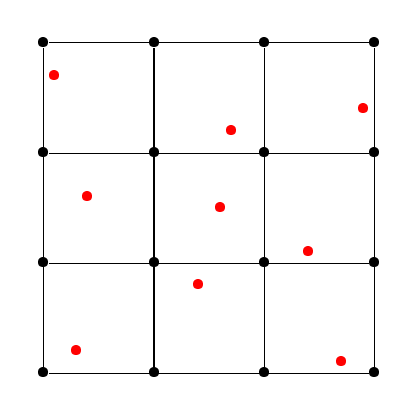
\begin{tikzpicture}[scale=0.7, x=2cm,y=2cm]
        \tikzset{c/.style = {shorten <=-4pt, shorten >=-4pt}}
        \tikzset{smalledge/.style = {-{Latex[length=2mm]},shorten <=-4pt}}
        
        \node (x1y1) at (0,0) {\textbullet};
        \node (x2y1) at (1,0) {\textbullet};
        \node (x3y1) at (2,0) {\textbullet};
        \node (x4y1) at (3,0) {\textbullet};

        \node (x1y2) at (0,1) {\textbullet};
        \node (x2y2) at (1,1) {\textbullet};
        \node (x3y2) at (2,1) {\textbullet};
        \node (x4y2) at (3,1) {\textbullet};

        \node (x1y3) at (0,2) {\textbullet};
        \node (x2y3) at (1,2) {\textbullet};
        \node (x3y3) at (2,2) {\textbullet};
        \node (x4y3) at (3,2) {\textbullet};

        \node (x1y4) at (0,3) {\textbullet};
        \node (x2y4) at (1,3) {\textbullet};
        \node (x3y4) at (2,3) {\textbullet};
        \node (x4y4) at (3,3) {\textbullet};

        \draw[c] (x1y1) edge node{} (x4y1);
        \draw[c] (x1y2) edge node{} (x4y2);
        \draw[c] (x1y3) edge node{} (x4y3);
        \draw[c] (x1y4) edge node{} (x4y4);

        \draw[c] (x1y1) edge node{} (x1y4);
        \draw[c] (x2y1) edge node{} (x2y4);
        \draw[c] (x3y1) edge node{} (x3y4);
        \draw[c] (x4y1) edge node{} (x4y4);

        \node[red] (s1) at (0.3,0.2) {\textbullet};
        \node[red] (s2) at (1.4,0.8) {\textbullet};
        \node[red] (s3) at (2.7,0.1) {\textbullet};
        \node[red] (s4) at (0.4,1.6) {\textbullet};
        \node[red] (s5) at (1.6,1.5) {\textbullet};
        \node[red] (s6) at (2.4,1.1) {\textbullet};
        \node[red] (s7) at (0.1,2.7) {\textbullet};
        \node[red] (s8) at (1.7,2.2) {\textbullet};
        \node[red] (s9) at (2.9,2.4) {\textbullet};

        \end{tikzpicture}
        \captionof{figure}{Voronoi grid with pseudo-randomly assigned seed points for each cell.}
        \label{img:tikz:noise:voronoi}
    \end{minipage}
    \hfill
    \begin{minipage}{0.47\linewidth}
        \centering
        \begin{tikzpicture}[scale=0.7, x=2cm,y=2cm]
            \tikzset{c/.style = {shorten <=-4pt, shorten >=-4pt}}
            \tikzset{smalledge/.style = {-{Latex[length=2mm]},shorten <=-4pt}}
            
            \node (gradient) at (1.5,1.5) {\includegraphics[width=4.2cm] {noise/2d voronoi unmixed}};

            \node (x1y1) at (0,0) {\textbullet};
            \node (x2y1) at (1,0) {\textbullet};
            \node (x3y1) at (2,0) {\textbullet};
            \node (x4y1) at (3,0) {\textbullet};

            \node (x1y2) at (0,1) {\textbullet};
            \node (x2y2) at (1,1) {\textbullet};
            \node (x3y2) at (2,1) {\textbullet};
            \node (x4y2) at (3,1) {\textbullet};

            \node (x1y3) at (0,2) {\textbullet};
            \node (x2y3) at (1,2) {\textbullet};
            \node (x3y3) at (2,2) {\textbullet};
            \node (x4y3) at (3,2) {\textbullet};

            \node (x1y4) at (0,3) {\textbullet};
            \node (x2y4) at (1,3) {\textbullet};
            \node (x3y4) at (2,3) {\textbullet};
            \node (x4y4) at (3,3) {\textbullet};

            \draw[c] (x1y1) edge node{} (x4y1);
            \draw[c] (x1y2) edge node{} (x4y2);
            \draw[c] (x1y3) edge node{} (x4y3);
            \draw[c] (x1y4) edge node{} (x4y4);

            \draw[c] (x1y1) edge node{} (x1y4);
            \draw[c] (x2y1) edge node{} (x2y4);
            \draw[c] (x3y1) edge node{} (x3y4);
            \draw[c] (x4y1) edge node{} (x4y4);

            \node[red] (s1) at (0.3,0.2) {\textbullet};
            \node[red] (s2) at (1.4,0.8) {\textbullet};
            \node[red] (s3) at (2.7,0.1) {\textbullet};
            \node[red] (s4) at (0.4,1.6) {\textbullet};
            \node[red] (s5) at (1.6,1.5) {\textbullet};
            \node[red] (s6) at (2.4,1.1) {\textbullet};
            \node[red] (s7) at (0.1,2.7) {\textbullet};
            \node[red] (s8) at (1.7,2.2) {\textbullet};
            \node[red] (s9) at (2.9,2.4) {\textbullet};

        \end{tikzpicture}
        \captionof{figure}{Voronoi grid with seed distances visualized.}
        \label{img:tikz:noise:voronoi2}
    \end{minipage}
\end{figure}

\noindent
As understandable, in \autoref{img:tikz:noise:voronoi2}, hard contours are still visible along the grid lines. This can be improved by including the adjacent cells when finding the closest seed for any given fragment.
This amounts to $3^n - 1$ neighboring cells, where $n$ is the number of dimensions. This means for 2D space its eight cells, while in 3D its 26.

\begin{figure}[H]
    \centering
    \begin{tikzpicture}[scale=1.2, x=2cm,y=2cm]
        \tikzset{c/.style = {shorten <=-4pt, shorten >=-4pt}}
        \tikzset{smalledge/.style = {-{Latex[length=2mm]},shorten <=-4pt}}
        
        \node (gradient) at (1.5,1.5) {\includegraphics[width=7.2cm] {noise/2d voronoi}};

        \node (x1y1) at (0,0) {\textbullet};
        \node (x2y1) at (1,0) {\textbullet};
        \node (x3y1) at (2,0) {\textbullet};
        \node (x4y1) at (3,0) {\textbullet};

        \node (x1y2) at (0,1) {\textbullet};
        \node (x2y2) at (1,1) {\textbullet};
        \node (x3y2) at (2,1) {\textbullet};
        \node (x4y2) at (3,1) {\textbullet};

        \node (x1y3) at (0,2) {\textbullet};
        \node (x2y3) at (1,2) {\textbullet};
        \node (x3y3) at (2,2) {\textbullet};
        \node (x4y3) at (3,2) {\textbullet};

        \node (x1y4) at (0,3) {\textbullet};
        \node (x2y4) at (1,3) {\textbullet};
        \node (x3y4) at (2,3) {\textbullet};
        \node (x4y4) at (3,3) {\textbullet};

        \draw[c] (x1y1) edge node{} (x4y1);
        \draw[c] (x1y2) edge node{} (x4y2);
        \draw[c] (x1y3) edge node{} (x4y3);
        \draw[c] (x1y4) edge node{} (x4y4);

        \draw[c] (x1y1) edge node{} (x1y4);
        \draw[c] (x2y1) edge node{} (x2y4);
        \draw[c] (x3y1) edge node{} (x3y4);
        \draw[c] (x4y1) edge node{} (x4y4);

        \node[red] (s1) at (0.3,0.2) {\textbullet};
        \node[red] (s2) at (1.4,0.8) {\textbullet};
        \node[red] (s3) at (2.7,0.1) {\textbullet};
        \node[red] (s4) at (0.4,1.6) {\textbullet};
        \node[red] (s5) at (1.6,1.5) {\textbullet};
        \node[red] (s6) at (2.4,1.1) {\textbullet};
        \node[red] (s7) at (0.1,2.7) {\textbullet};
        \node[red] (s8) at (1.7,2.2) {\textbullet};
        \node[red] (s9) at (2.9,2.4) {\textbullet};

    \end{tikzpicture}
    \captionof{figure}{Complete 2D Voronoi noise pattern.}
    \label{img:tikz:noise:voronoi3}
\end{figure}

\pagebreak

\noindent
An implementation of this relatively simple algorithm could look like the following listing.
\begin{lstlisting}[language=HLSL, caption=Implementation of 2D Voronoi noise algorithm., label=lst:shader:noise:voronoi2d]
float2 randomSeed(float2 co) {
    return float2(
        fract(sin(dot(co, float2(12.9898, 78.233))) * 43758.5453123),
        fract(sin(dot(co, float2(39.3461, 11.135))) * 14375.8545359));
}

float voronoi(float2 p) {
    float2 baseCell = floor(p);
    float dMin = 999;

    for(int x = -1; x <= 1; x++) {
        for(int y = -1; y <= 1; y++) {
            float2 cell = baseCell + float2(x, y);
            float2 seed = cell + randomSeed(cell);
            float d = distance(seed, p);
            if (d < dMin) {
                dMin = d;
            }
        }
    }
    
    return dMin;
}
\end{lstlisting}

\noindent
The 3D equivalent of the algorithm looks fairly similar.

\begin{lstlisting}[language=HLSL, caption=Implementation of 3D Voronoi noise algorithm., label=lst:shader:noise:voronoi3d]
float3 randomSeed(float3 co) {
    return float3(
    fract(sin(dot(co, float3(12.989, 78.233, 37.719))) * 43758.5453123),
    fract(sin(dot(co, float3(39.346, 11.135, 83.155))) * 14375.8545346),
    fract(sin(dot(co, float3(73.156, 52.235, 09.151))) * 31396.2234116));
}

float voronoi(float3 p) {
    float3 baseCell = floor(p);
    float dMin = 999;

    for(int x = -1; x <= 1; x++) {
        for(int y = -1; y <= 1; y++) {
            for(int z = -1; z <= 1; z++) {
                float3 cell = baseCell + float3(x, y, z);
                float3 seed = cell + randomSeed(cell);
                float d = distance(seed, p);
                if (d < dMin) {
                    dMin = d;
                }
            }
        }
    }
    
    return dMin;
}
\end{lstlisting}

\subsection{Seamless Noise}
\label{section:noise:seamless}

\subsection{Compute Shaders}
\label{section:noise:compute}

\subsection{3D Noise Texture Sampling}
\label{section:noise:tex3d}